\chapter{Implementación}
\label{cap:Implementacion}



\section{Herramientas y Librerías: \textit{stack} tecnológico}

La figura XX muestra las librerias.... \textcolor{red}{redactar y ver si falta alguna}

\begin{table}[hbt!]
\centering
\renewcommand{\arraystretch}{1.3} % Da un poco de espacio vertical a las celdas
\begin{tabular}{|l|l|p{10cm}|}
\hline
\textbf{Biblioteca} & \textbf{Versión} & \textbf{Dónde se usa} \\
\hline
\texttt{torch} & 2.5.1 & Definición del modelo, capas CNN, funciones de pérdida, optimizador Adam, backpropagation y guardado de checkpoints. \\
\hline
\texttt{torchaudio} & 2.5.1 & Carga de WAV, transformadas Spectrogram, MelSpectrogram, AmplitudeToDB. \\
\hline
\texttt{librosa} & 0.11.0 & Carga de audio en inferencia, visualización de espectrogramas con eje logarítmico (\texttt{specshow}). \\
\hline
\texttt{numpy} & 2.2.6 & Síntesis FM, generación de envolventes, operaciones con arrays en evaluación y desnormalización. \\
\hline
\texttt{sounddevice} & 0.5.3 & Reproducción de audio en tiempo real y stream del sintetizador interactivo. \\
\hline
\texttt{soundfile} & 0.13.1 & Escritura de WAVs del dataset y lectura para reproducción. \\
\hline
\texttt{matplotlib} & 3.10.8 & Gráficas de evaluación y ventana de comparación de espectrogramas. \\
\hline
\texttt{scikit-learn} & 1.7.2 & Dependencia transitiva de librosa (no usado directamente en el código principal). \\
\hline
\texttt{tkinter} & 8.6.13 & GUI completa: páginas de inicio, entrenamiento y test; sintetizador interactivo. \\
\hline
\texttt{ffmpeg} & $\ge$ 8.0 & Backend de torchaudio para decodificación de audio; instalado vía conda para garantizar compatibilidad en Windows. \\
\hline
\end{tabular}
\caption{Bibliotecas principales utilizadas en el proyecto.}
\label{tab:stack_tecnologico}
\end{table}

\section{\textit{Pipeline} de Entrenamiento}

Se adjunta la Figura~\ref{fig:workflow_v5.2} con el objetivo de facilitar la comprensión del modelo 
del Prototipo 5. El trabajo queda dividido en 5 fases: generación de audio, conversión a tensores, 
preparación del dataset, entrenamiento (con múltiples opciones de arquitectura) e inferencia paramétrica.
\begin{figure} 
    \centering
    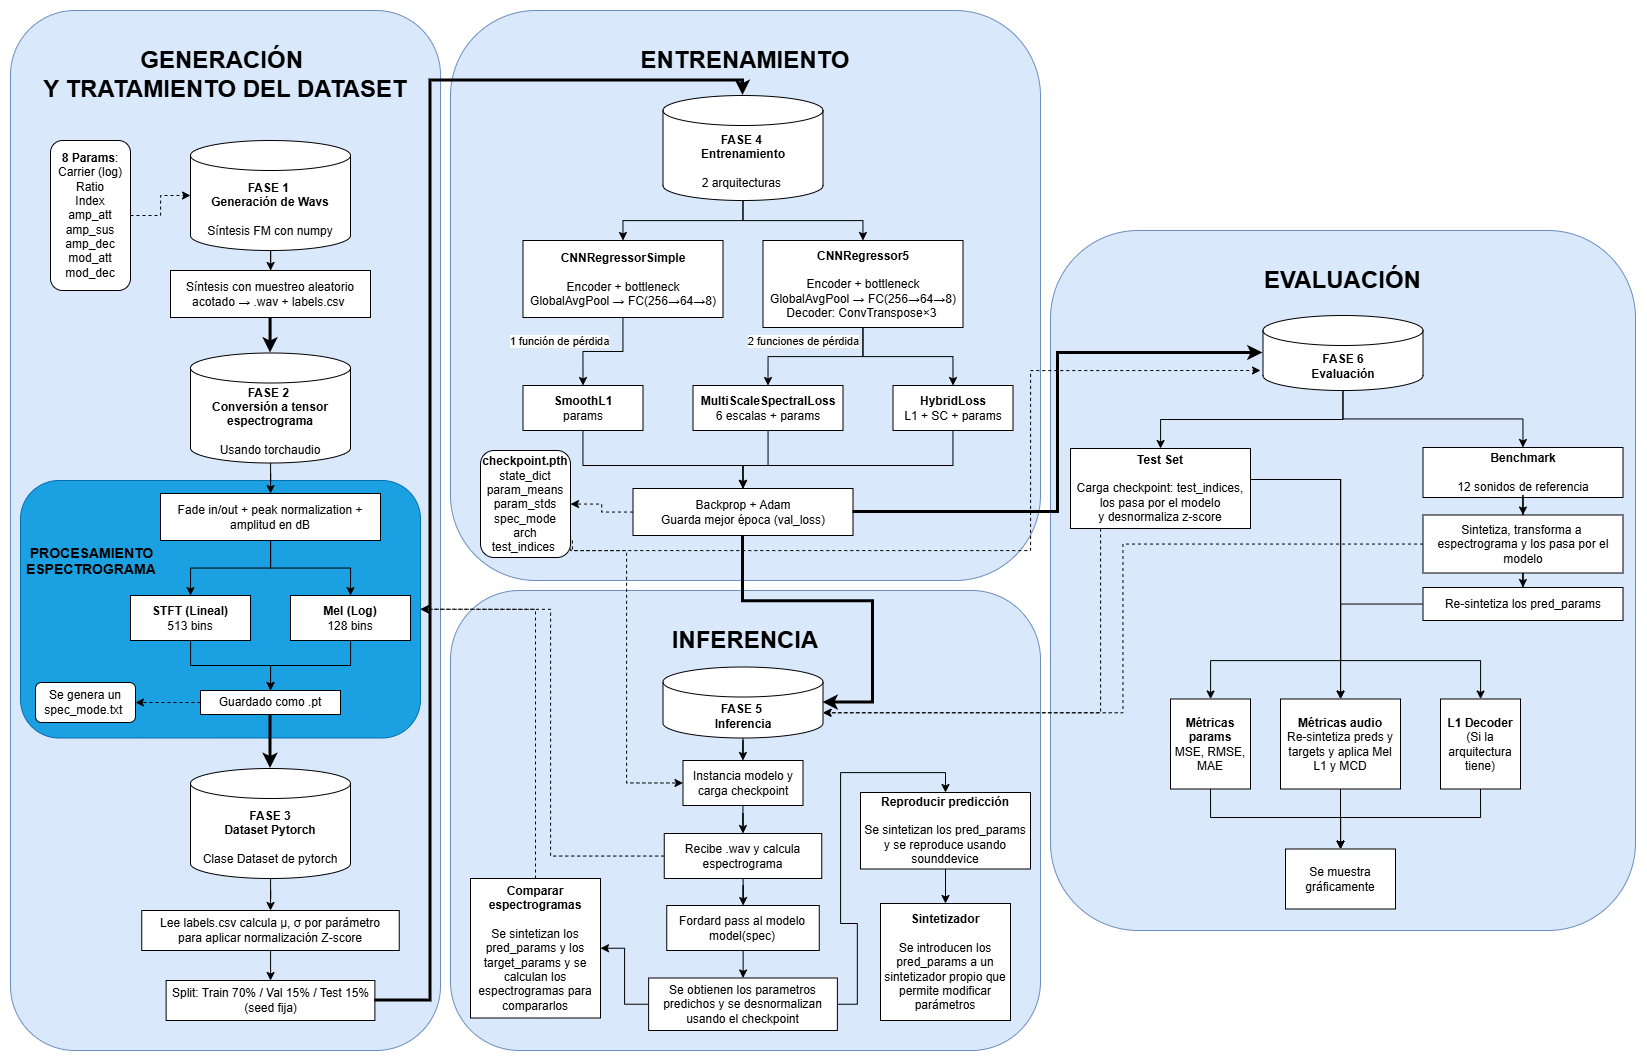
\includegraphics[width=1\textwidth]{Imagenes/Bitmap/diagrama}
    \caption{Flujo de trabajo del Modelo: desde la síntesis matemática hasta la inferencia y evaluación del modelo.}
    \label{fig:workflow_v5.2}
\end{figure}

Como se muestra en el diagrama \ref{fig:workflow_v5.2}, en primer lugar se encuentra la generación y tratamiento del dataset. La generación se lleva acabo de la manera especificada en el punto \ref{sec:GeneracionDataset} y se preprocesa (\ref{sec:Preprocesamiento}). Tras esto, el dataset ya está preparado y dividido de tal forma que se tiene un conjunto de entrenamiento que se utilizará en la siguiente fase. 

La fase de entrenamiento (fase 4 del diagrama \ref{fig:workflow_v5.2}) comienza con la elección de la arquitectura y función de pérdidas (descritas en \ref{sec:ArquitecturaCNN} y \ref{sec:FuncionPerdida} respectivamente). Y, en la etapa final, se encuentra el algoritmo de retropropagación (\textit{Backpropagation}), mediante el cual se actualizan
los pesos para así minimizar el error en la red, calculando los gradientes del error con respecto a cada nodo. 
Para la actualización de los pesos se emplea el optimizador \textbf{Adam} (\textit{Adaptive Moment Estimation}). Este se elige frente al descenso de gradiente común (SGD) debido al cálculo que hace 
de las tasas de aprendizaje adatativas e independientes para cada parámetro. A parte, se guardan los pesos de la época que ha conseguido 
el mínimo histórico con respecto al error sobre el conjunto de validación. Estos valores se almacenan en un archivo de punto de control (checkpoint.pth) junto
con el resto de información de contexto necesaria: 

\begin{itemize}
        \item \textbf{Parámetros de Desnormalización: } Contiene las medias y desviaciones estándar obtenidas en la Fase 3 del diagrama
        sobre los parámetros. Estas son necesarias para poder revertir el Z-score en las futuras predicciones. 
          
        \item \textbf{Contexto de Arquitectura: } Son las etiquetas que describen la topología (\textit{arch}: simple o full)
        y el tipo de espectrogramas (\textit{spec\_mode}: stft o mel) que se han utilizado para el modelo.
        
        \item \textbf{Aislamiento de Datos: } Contiene los índices del conjunto de prueba (\textit{test\_indices}), necesario para la evaluación.
        

\end{itemize}

Una vez terminados todos estos procesos, el modelo ya se encuentra entrenado y listo para inferir parámetros o ser evaluado.

\section{Inferencia de parámetros} 
La fase 5 (del diagrama anterior) consiste en la inferencia de parámetros de síntesis FM, mediante el modelo entrenado previamente, a partir
de audios. 

Al inicio de esta fase, se carga el punto de control que instancia automáticamente el tipo de red. 

La inferencia comienza cuando se recibe un archivo de audio (\textit{.wav}). En ese momento, se sigue el mismo flujo
que en la Fase 2, transformando el audio en un tensor de espectrograma (del tipo indicado por \textit{spec\_mode}). Este 
se introduce en el modelo (\textit{forward pass}), obteniendo así un vector latente de 8 valores, sobre el que se aplica
una desnormalización (con los valores de Z-score almacenados en el \textit{checkpoint}) que da como resultado la predicción de 
los parámetros. 

En este punto, el sistema te permite llevar a cabo varias acciones diferentes mediante la 
interfaz gráfica (GUI). Por un lado, se puede realizar una comparación visual del espectrograma del audio
predicho con el del audio original. Para ello, se sintetizan los parámetros obtenidos y los parametros originales y se 
calculan sus espectrogramas. También se da la opción de comparar acústicamente el audio original con el sintetizado por los parámetros
inferidos (mediante \textit{sounddevice}) y de exportar estos a un sintetizador propio, con la opción de modificarlos manualmente. 

\section{Interfaz Gráfica de la aplicación}
Para una mejor experiencia de uso y facilitar el entorno de entrenamientos y pruebas de la aplicación, se ha desarrollado una Interfaz Gráfica. Se trata de una serie de pantallas sencillas, programadas en Python mediante el uso de la librería \textit{Tkinter}.

En la primera pantalla (\ref{fig:pantalla1}), se da la opción de elegir un modelo existente o de entrenarlo. 

En caso de decidir cargar un modelo, se podrá seleccionar mediante el explorador de archivos. A continuación (\ref{fig:pantallaPruebas}), existen dos posibilidades: probar predicciones independientes de audios o realizar una evaluación general. En la primera, se puede cargar un wav y generar una predicción, existiendo la posibilidad de compararlos auditivamente o gráficamente sus espectrogramas (en frecuencia lineal y en logarítmica) y de ejecutar un sintetizador. En la pantalla del sintetizador(\ref{fig:sinte}), aparecen los parámetros de la predicción y los del audio original (en caso de tenerlos), siendo modificables. Además, el teclado hace la función de teclas del sintetizador con el sonido generado por los parámetros seleccionados. 

La sección del entrenamiento (\ref{fig:pantallaEntrenamiento}) es la dedicada a seleccionar varios aspectos relevantes, tanto para el tiempo y forma de entrenamiento como para la topología del modelo. Por un lado, se permite elegir si entrenar el modelo en CPU o en GPU, lo que afectará directamente a su tiempo de entrenamiento. Por el otro, hay que decidir que tipo de espectrograma, arquitectura del modelo y función de pérdida (explorados en el apartado anterior) van a ser los que definan el modelo. El siguiente campo de la pantalla incluye la opción de crear el dataset (explicado anteriormente) o cargar uno personalizado. En último lugar se encuentra el apartado de parámetros modificables para el entrenamiento, como son las épocas (\textit{epoch}), la tasa de aprendizaje (\textit{Learning Rate}) y los pesos de los parámetros de las funciones de pérdida. 

\section{Estructura del Código}

Para asegurar la mantenibilidad y escalabilidad, el código se estructura mediante el principio de Separación de Responsabilidades (\textit{Separation of Concerns}). Se divide así la aplicación en dos módulos diferentes:

\begin{itemize}
    \item \textbf{Lógica (Backend): } Se encuentra en el archivo {\textit{logica.py}}. Aquí se agrupan las funciones matemáticas para la síntesis, calculo de métricas, generación de espectrogramas, etc. 
    \item \textbf{Vista y Controlador (Frontend): } Archivo \textit{main.py}. Este implementa la interfaz, recibe los \textit{inputs} del usuario y gestiona el flujo de llamadas a la lógica y los errores.
\end{itemize}

Adicionalmente, destaca el uso de la Programación Orientada a Objetos (POO) y el encapsulamiento. Estas características se aplican en la aplicación de la siguiente manera:

\begin{itemize}
    \item \textbf{Clase App (\textit{main.py}): } Se encarga de encapsular el estado global. Evita el uso de variables globales manteniendo las variables necesarias instanciadas en esta clase (\textit{self.dataset\_obj}, \textit{self.pathModelo}, \textit{self.model\_trained}, etc).
    \item \textbf{Clase SpectrogramTensorDataset (\textit{dataset.py}): } Hereda de la clase base de \textit{Pytorch} de \textit{torch.utils.data.Dataset}, teniendo acceso a métodos como el de procesamiento por lotes (\textit{batching}). Asimismo, esta clase se encarga de los cálculos de estadísticas de normalización y mapeo de los archivos, de forma que desde fuera se obtienen los datos ya preparados mediante el método \textit{\_\_getitem\_\_}. 
    \item \textbf{Modelos y Funciones de Pérdida: } Como se ha mencionado previamente, existen diferentes arquitecturas y funciones de pérdida y todas ellas heredan de \textit{nn.Modules}. En consecuencia, el código permite que la lógica del entrenamiento sea independiente del modelo exacto que se esté utilizando, lo que se conoce como \textbf{Polimorfismo}. Por otro lado, la clase \textit{HybridLoss} encapsula la lógica de la convergencia espectral y la norma de Frobenius, manteniendo el entrenamiento ajeno a estas fórmulas. 
    \item \textbf{\textit{FMSynth8Window}: } La pantalla del sintetizador se encuentra totalmente desacoplada del resto de la lógica, siendo una clase independiente. De esta manera, se puede utilizar tanto desde la ejecución normal de la aplicación como de forma aislada, facilitando así su construcción, ampliación y pruebas aisaldas.
    

\end{itemize}


\begin{figure} 
    \centering
    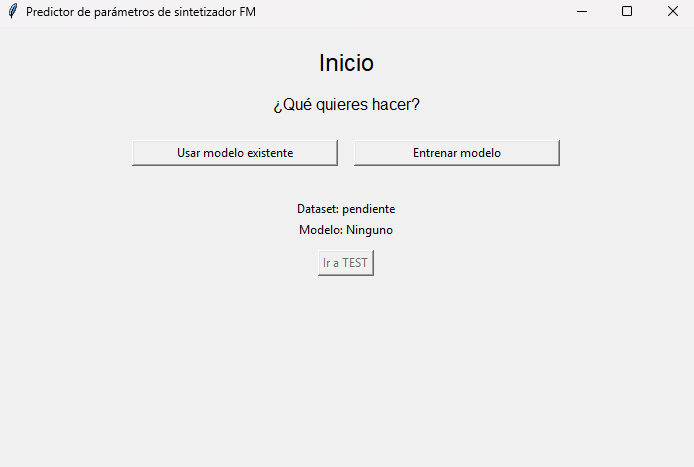
\includegraphics[width=1\textwidth]{Imagenes/Bitmap/pantalla1}
    \caption{Primera pantalla de la Interfaz Gráfica de la Aplicación, elección uso modelo o entrenamiento.}
    \label{fig:pantalla1}
\end{figure}

\begin{figure} 
    \centering
    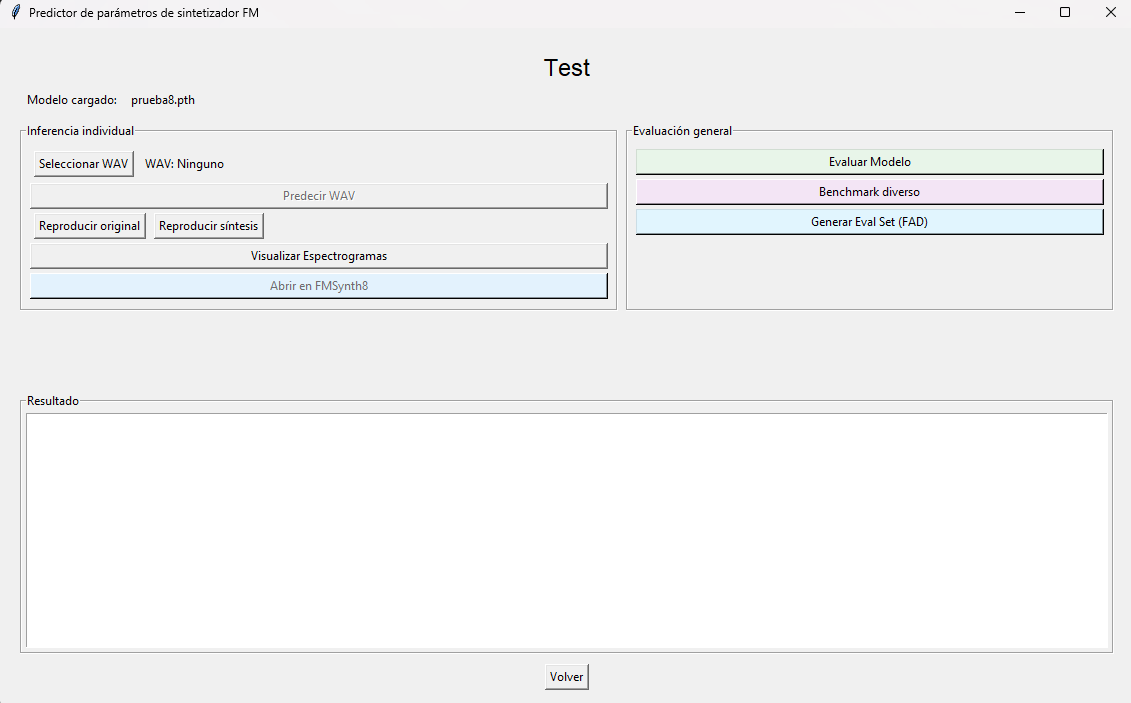
\includegraphics[width=1\textwidth]{Imagenes/Bitmap/pantallaPruebas}
    \caption{Pantalla en la que se pueden hacer pruebas con el modelo seleccionado.}
    \label{fig:pantallaPruebas}
\end{figure}

\begin{figure} 
    \centering
    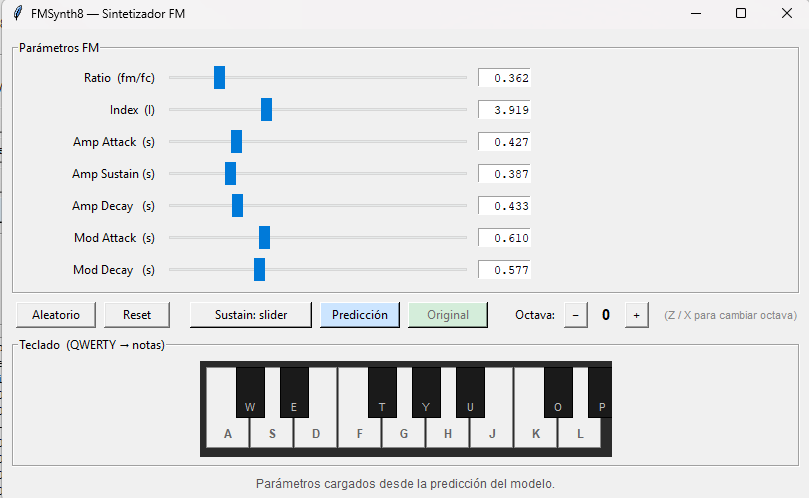
\includegraphics[width=1\textwidth]{Imagenes/Bitmap/sinte}
    \caption{Sintetizador FM de prueba.}
    \label{fig:sinte}
\end{figure}

\begin{figure} 
    \centering
    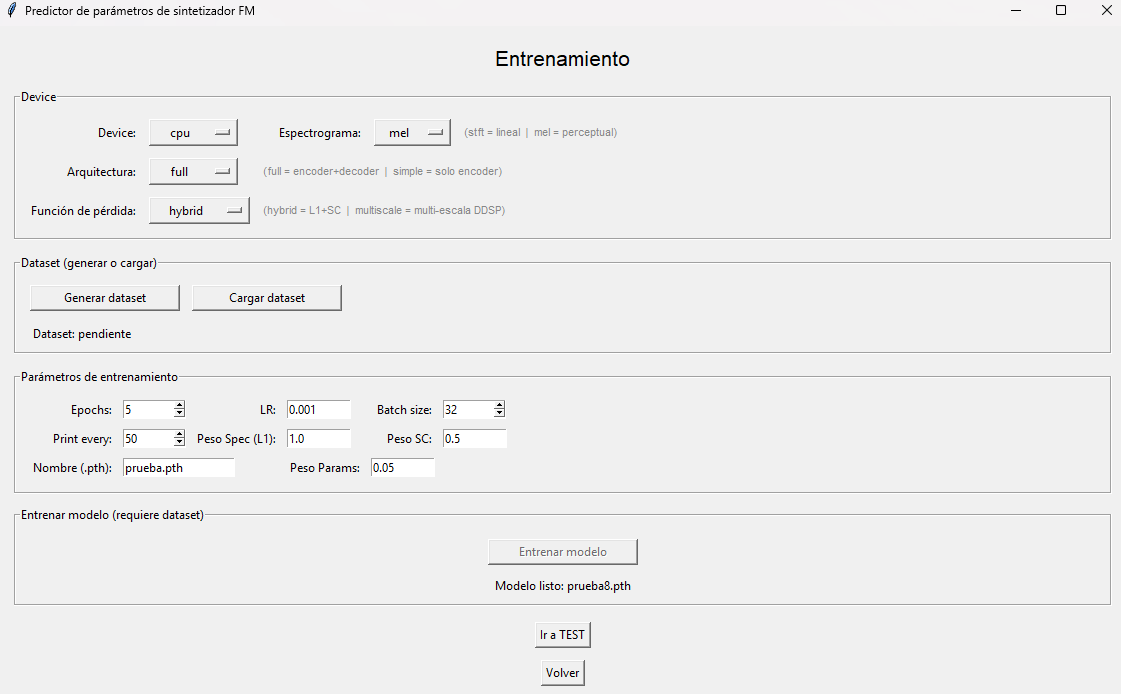
\includegraphics[width=1\textwidth]{Imagenes/Bitmap/pantallaEntrenamiento}
    \caption{Sintetizador FM de prueba.}
    \label{fig:pantallaEntrenamiento}
\end{figure}

